\documentclass{article} % For LaTeX2e
\usepackage{nips15submit_e,times}
\usepackage{hyperref}
\usepackage{url}
\usepackage{graphicx}
%\documentstyle[nips14submit_09,times,art10]{article} % For LaTeX 2.09


\title{Fully Convolutional Networks for Semantic
Segmentation}

\author{
Nan Wei \\
UC San Diego\\
\texttt{nwei@ucsd.edu} \\
\And
Renjie Shao \\
UC San Diego \\
\texttt{reshao@ucsd.edu} \\
\And
Hongyi Ling \\
UC San Diego \\
\texttt{holing@ucsd.edu} \\
}

% The \author macro works with any number of authors. There are two commands
% used to separate the names and addresses of multiple authors: \And and \AND.
%
% Using \And between authors leaves it to \LaTeX{} to determine where to break
% the lines. Using \AND forces a linebreak at that point. So, if \LaTeX{}
% puts 3 of 4 authors names on the first line, and the last on the second
% line, try using \AND instead of \And before the third author name.

\newcommand{\fix}{\marginpar{FIX}}
\newcommand{\new}{\marginpar{NEW}}

\nipsfinalcopy % Uncomment for camera-ready version

\begin{document}


\maketitle

\begin{abstract}

\end{abstract}

\section{Introduction}


\section{Method}

\begin{figure}[htb!]
    \centering
     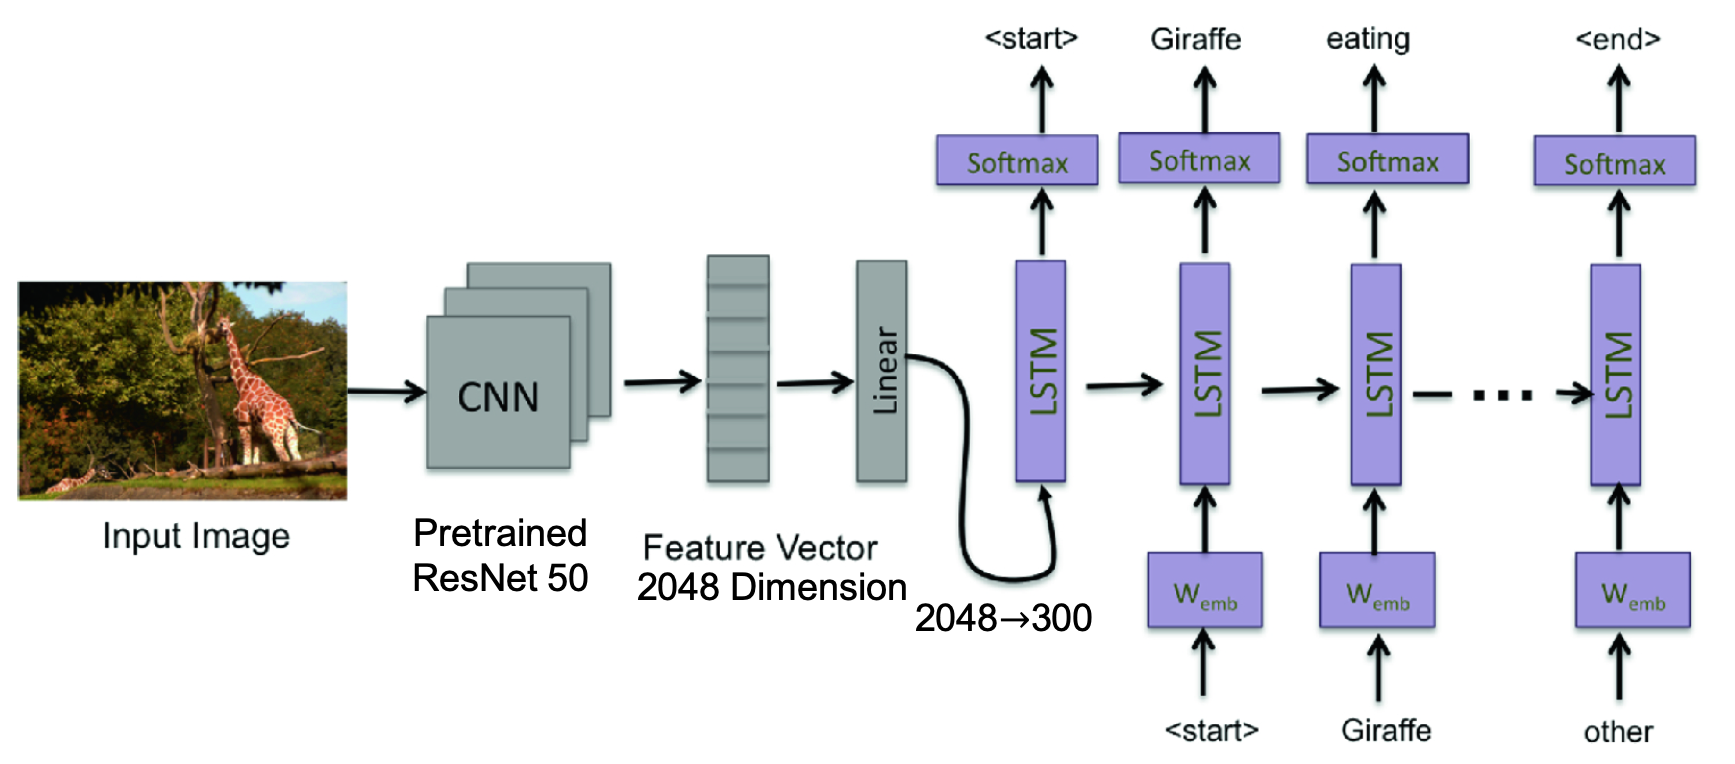
\includegraphics[width=0.8\textwidth]{frame}
    \caption{Model Framework \cite{10.1007/978-3-030-04780-1_23}}
    \label{loss_fcn}
\end{figure}

\section{Experiments}

\begin{figure}[htb!]
    \centering
     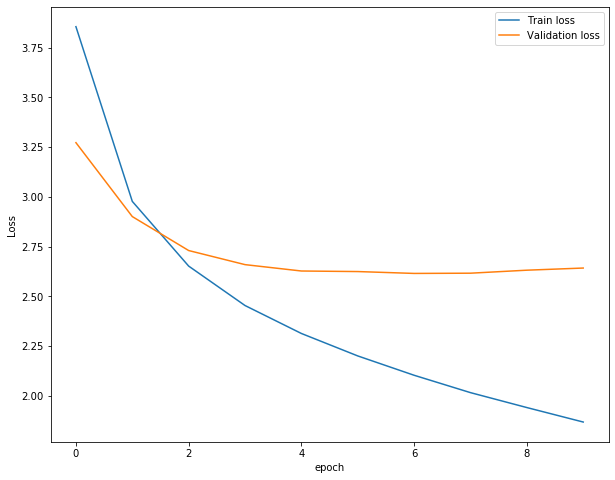
\includegraphics[width=0.8\textwidth]{RNNloss}
    \caption{Training and validation loss of vanilla RNN}
    \label{loss_fcn}
\end{figure}



\section{Individual Contribution}

\subsection*{Nan Wei}
I implement transfer learning with DeepLabv3 and do experiments on basic CNN and DeepLabv3. I also write the report.

\subsection*{Renjie Shao}
I implement U-Net architecture and do experiments on U-Net. I also help implement IoU and visualization of segmentation and write some parts of the report.
\subsection*{Hongyi Ling}
I write the code of basic fcn and metrics. I also build different experimental CNN architectures and test these neural networks. In addition, I write these parts of the report.

\bibliographystyle{unsrt}
\bibliography{references}


\end{document}
